\section{What is aging?}


\subsection{Definition and Hallmarks}

\begin{frame}[c]{Aging}
    \large

    \begin{block}{Definition}
        Aging is characterized by progressive decline in tissue and organ
        function and increased risk of mortality. From \cite{sen2016epigenetic}
    \end{block}
    \pause
    But how can we measure it?
\end{frame}


\begin{frame}[c]{Hallmarks of Aging}
    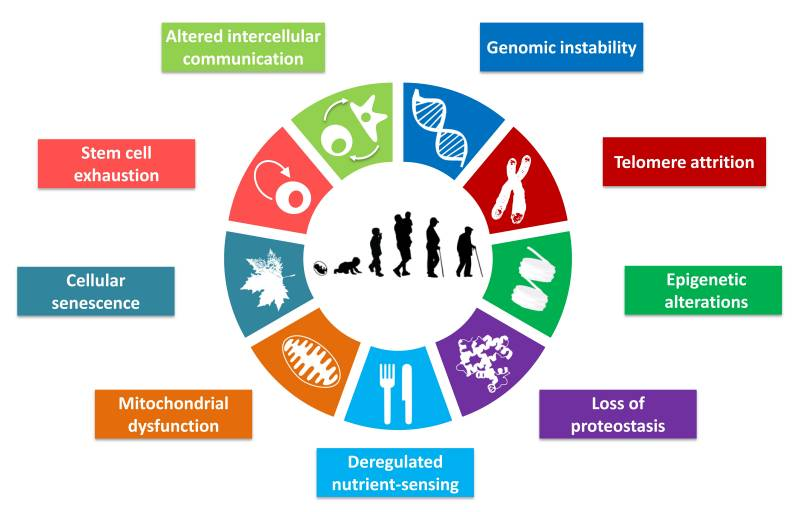
\includegraphics[width=\textwidth]{hallmarks_aging} \\
    \cite{lopez2013hallmarks}
    % \begin{itemize}[<+(1)->]
    %     \item Genomic instability
    %     \item Telomere attrition
    %     \item Epigenetic alterations
    %     \item Loss of proteostasis
    %     \item Deregulated nutrient-sensing
    %     \item Mitochondrial dysfunction
    %     \item Cellular senescence
    %     \item Stem cell exhaustion
    %     \item Altered intercellular communication
    % \end{itemize}
\end{frame}



